
\begin{savequote}[10pc]
\sffamily
``If you have built castles in the air, your work need not be lost; that is where they should be. Now put the foundations under them.''
\qauthor{Henry David Thoreau \\(1817 -- 1862)}
\end{savequote}
\chapter{The We Love Wind Web Service}\label{chap:gae_ws}
In this chapter we describe the implementation of the corner stone in the We Love
Wind application: the We Love Wind Web Service. We implement the service using
Google App Engine/Django, described in Chapter~\ref{chap:gae}.

The last chapter covered all the resources of the Web Service; we now turn to the
logic backing the resources. Since the architecture is a typical MVC
architecture, the implementation is presented in terms of this style.

The interested reader can access the Web Service by pointing a browser to the
following URIs:
\begin{itemize}
  \item \url{http://www.welovewind.com/api/spots/}
  \item \url{http://www.welovewind.com/api/weather_stations/}
  \item \url{http://www.welovewind.com/api/forecast_points/}
\end{itemize}

\section{Implementation of Models}\label{sec:models}

\begin{figure}[htbp]
  \centering
  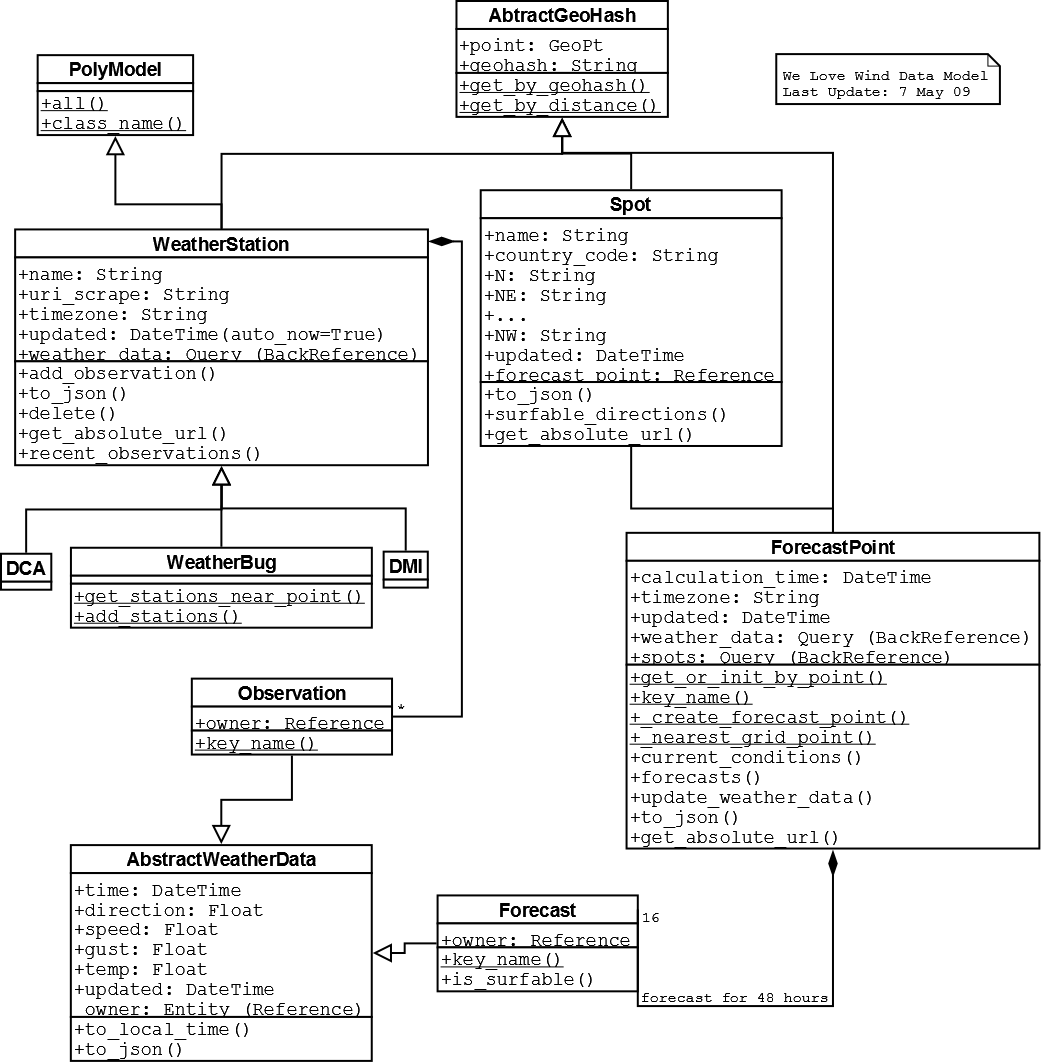
\includegraphics[width=\textwidth]{./Figures/DataModel}
  \caption{Data model (UML notation)}
  \label{fig:data_model}
\end{figure}

The models are not just defining the structure of data; the models contain all
the business logic of the application separating and encapsulating the data of
the application from the presentation of it.

Figure~\ref{fig:data_model} shows the data models of the application in a UML
static structure diagram. Arguments to methods is left out for brevity. Methods
underlined in the diagram are Python class methods. Since all data models inherit
from the \verb|db.Model| class it is omitted. The figure is a good mental model
to have in mind during the descriptions of the different model classes.

%%%%%%%
\subsection{AbstractGeoHash model}
Listing~\ref{lst:geohashmodel} shows the AbstractGeoHash model. The purpose of
the model is to provide geohash structure and logic for any model that inherits
from it; in that way all properties and methods relevant for geohashing is
factored out of the other models, i.e., spot, weather station, and forecast point.

\subsubsection*{Structure}
The model contains two properties: \verb|point| and \verb|geohash|. Point is the
 latitude and longitude for a place, and geohash is the geohash encoding of the
 latitude and longitude.

\subsubsection*{Logic}
The model contains logic that gets all points of the current class that have the
same geohash prefix as the given: manifested in \verb|get_near_geohash|. GQL
lacks the option to search for patterns in strings (\verb|LIKE| in SQL), instead
two inequality filter are applied to match the geohash prefix pattern; the last
filter sets the upper boundary of the range of results to return since the prefix
is concatenated with the largest possible unicode character: the replacement
character which is encoded as
\verb|u"\ufffd"|.\footnote{\url{http://en.wikipedia.org/wiki/Replacement_character}}

In addition, the model includes logic which retrieves all points within a
threshold distance of a given point: manifested in \verb|get_near_point|.  It
applies the geohash neighbors technique to get neighbors. The method uses
\verb|get_near_geohash| to get all points in the geohash areas; afterward pruning
the list to points within the threshold. Currently, the method assumes that the
radius (distance) from the center point is within the geohash neighbors.

Instances of the \verb|GeoHash| model automatically get a geohash value, since
the \verb|put| method is overwritten, and before saving the instance to the
datastore the geohash value is calculated and set. 

\begin{lstlisting}[caption=GeoHash model, label=lst:geohashmodel]
class AbstractGeoHash(db.Model):
    
    point = db.GeoPtProperty(required=True)
    geohash = db.StringProperty()
    
    @classmethod
    def get_near_geohash(cls, ghash_prefix, geohash_offset):
        ghash_prefix = ghash_prefix.lower()
        query = db.Query(cls)
        query.filter('geohash >=', geohash_offset)
        query.filter('geohash <', ghash_prefix + u"\ufffd")
        return query
    
    @classmethod
    def get_near_point(cls, point, distance, geohash_prefix_length = 3):
        entities = []
        center = geohash.encode(point.lat, point.lon)[:geohash_prefix_length]
        ghashes = geohashneighbors.neighbors(center)
        ghashes.append(center)
        
        for h in ghashes:
            query = cls.get_near_geohash(h,h)
            for entity in query:
                entities.append(entity)

        def prune(list):
            '''Prune a sorted list by distance'''
            for i, point in enumerate(list):
                if point.distance > distance:
                    return list[:i]
            return list
        
        return prune(geo.sort_by_distance(point, entities))
            
            
    def put(self):
        self.geohash = geohash.encode(self.point.lat, self.point.lon)
        return super(AbstractGeoHash, self).put()
\end{lstlisting}

%%%%%
\subsection{Spot model}
Listing~\ref{lst:spot_model} shows the Spot model. 

\subsubsection*{Structure}
The spot model inherits from the \verb|AbstractGeoHash| model: getting both a
\verb|point| and a \verb|geohash| property. Every spot has a \verb|name|, and, as
discussed in the resource section, every spot belongs to the nearest
\verb|forecast_point|. The many-to-one relationship between spots and forecast
points is implemented with the reference property.  The wind diagram is defined
as string attributes that must have one of four values: NO, MAYBE, YES, or
UNDEFINED.

The model has an updated property which is a pervasive property in
the data models. The property is automatically updated to the current datetime
each time the model is saved. This is useful for tracking the times of last
modification of entities, e.g., essential for implementing HTTP caching.

\subsubsection*{Logic}
There are two pervasive methods located on concrete models: \verb|to_json| and
\\\verb|get_absolute_url|. The \verb|to_json| method returns a simple Python object
representation of the instance ready for JSON serialization. The method will
prove its worth when we construct resource representations in the controllers in
Section~\ref{sec:controllers}.

The \verb|get_absolute_url| method return the URI for the concrete model; the
advantage is that changing the URI can now be done by just changing that method,
instead of refactoring all views.

As in the case with the \verb|AbtractGeoHash| model, the \verb|put| method is
overwritten to wire in some data. After saving a spot it is always associated
with the nearest forecast point and, in addition, the geohash value is wired into
the spot.

\begin{lstlisting}[caption=Spot model, label=lst:spot_model]
class Spot(AbstractGeoHash):
    WIND_DIAGRAM_CHOICES = ('NO','MAYBE', 'YES', 'UNDEFINED') 
    
    name = db.StringProperty(required=True)
    updated = db.DateTimeProperty(auto_now=True)
    country_code = db.StringProperty(required=True)
    forecast_point = db.ReferenceProperty(ForecastPoint, collection_name='spots')
    
    # wind diagram
    N  = db.StringProperty(default='UNDEFINED', choices=WIND_DIAGRAM_CHOICES)
    (...)
    NW = db.StringProperty(default='UNDEFINED', choices=WIND_DIAGRAM_CHOICES)
    
    def put(self):
        self.forecast_point = ForecastPoint.get_or_init_by_point(self.point)
        return super(Spot, self).put()
    
    @classmethod
    def key_name(self, country_code, name):
        return '/spots/%s/%s/' % (country_code, name)
    
    def to_json(self):
        return {
            'name':self.name,
            'country_code':self.country_code,
            'lat': self.point.lat,
            'lon': self.point.lon,
            'wind_diagram': self.surfable_directions(),
            'uri': self.get_absolute_url(),
            'forecast_point': self.forecast_point.get_absolute_url()
        }
        
    def get_absolute_url(self):
        return self.key().name()
(...)
\end{lstlisting}


\subsection{AbstractWeatherData Model}\label{sec:abstractweatherdatamodel}
The \verb|AbstractWeatherData| model, shown in
Listing~\ref{lst:abstract_weather_data_model} is a common supermodel for
forecasts and observations. Forecasts and observations have similar structure
except for the fact that forecasts belong to a forecast point and observations
belong to a weather station.

\subsubsection*{Structure}
The WeatherData model contains all the relevant weather data types mentioned
before: \verb|speed|, \verb|gust|, \verb|temp|, \verb|direction|, and a
\verb|time| of when the weather data applies. The model is abstract delegating
the references to its subclasses: Observation and Forecast. 

\begin{lstlisting}[caption=AbstractWeatherData model,label=lst:abstract_weather_data_model]
 class AbstractWeatherData(db.Model):
    '''Abtract weather data model.
    
    Attributes:
        is_new: indicates if this model is just created. Used by update_or_insert()
    
    Properties:
        updated: time of update on this server
        time: the observation / forecast time
    '''
    updated = db.DateTimeProperty(auto_now=True)
    direction = db.FloatProperty()
    speed = db.FloatProperty()
    temp = db.FloatProperty()
    gust = db.FloatProperty()
    time = db.DateTimeProperty(required=True)
    #abstract owner = db.ReferenceProperty()
    
    def __init__(self, is_new = False, **kwds):
        self.is_new = is_new
        super(AbstractWeatherData, self).__init__(**kwds)
        
    @classmethod
    def update_or_insert(cls, **kwds):
        key_name = cls.key_name(**kwds)
        entity = super(AbstractWeatherData, cls).get_or_insert(key_name, is_new=True, **kwds)
        if not entity.is_new:
            for prop in kwds.keys():
                setattr(entity, prop, kwds[prop])
            entity.put()
        return entity
(...)
\end{lstlisting}

\subsubsection*{Logic}
In an environment where weather data is continuously added eventually the
datastore will fill up. The datastore limit demands that some house keeping is
done. GAE cron jobs are limited in their number and duration time
\citep{Google:cron} and are not a scalable solution. An alternative to cleaning
up the datastore with cron jobs is needed.

An idea is continuously maintaining the datastore as new data is fed into it by
throwing out the oldest data. If we let, e.g., the last 24 hours of observations
and only the forecasts from the last calculation be in the datastore the amount
of weather data is pruned.

We let the weather data have a unique property, pertaining to the owner (weather
station or forecast point) and the time, e.g., a time delta such as total time of
day in minutes. When these properties are unique, inserting new data with the
same time delta and owner updates the existing entity. Implementation of unique
properties in the context of forecasts was presented in
Section~\vref{sec:unique_props}.

If the incoming data is consistently produced at certain times of the day the
technique is \textit{\gls{gls:fifo}} with a buffer size proportional to the
number of atomic units in the maximum time delta. In the case of observations the
buffer size is one day and the unit size is in minutes; that gives a maximum of
60 minutes * 24 hours = 1440 entities in the datastore per weather station. In
the case of forecasts the buffer size is 48 hours, however, since the time of
forecasts are always in hours the unit size is in hours; that gives a maximum of
48 entites per forecast point.

%% There are a total of 90 wind icons in the application. A certain wind icon is valid
%% for a certain speed interval and certain direction
%% interval. \verb|_direction_interval| maps from a direction number to a direction
%% string, which is the first part of the icon name. \verb|_speed_interval|
%% maps from the speed to a string indicating the interval the speed belongs to, the
%% last part of the icon name. \verb|wind_icon|, using that two methods, creates the
%% path to the icon representing the weather data.

\subsection{WeatherStation Model}\label{sec:ws_model}
Listing~\ref{lst:weather_station_model} shows the WeatherStation model. 

\subsubsection*{Structure}
The model inherits from the \verb|PolyModel| and the \verb|AbstractGeohash|. The
\verb|PolyModel| class provides a programmatic implementation of object
inheritance in the datastore similar to using NULL values to combine hierarchy
relations in relational databases \citep[sec.4.6]{db:Garcia-Molina:08}. The
advantage is that a query on the superclass includes all the entities from the
subclasses, and a query on the subclass only includes entities from the subclass.
The model has a list of observations. This is not visible in the model since it
is the reference property in the observation model that defines the one-to-many
relationship between weather stations and observations.

\subsubsection*{Logic}
The model is the owner of weather observations. As mentioned we overwrite
those observations on a circular basis. The model includes a method,\\
\verb|update_or_insert_observation|, that takes an observation resource in
deserialized JSON format and either inserts the observation or overwrites an
existing based on the unique properties of the observation model.


\begin{lstlisting}[label=lst:weather_station_model,caption=WeatherStation model]
class WeatherStation(polymodel.PolyModel, AbstractGeoHash):
 """Super model class for weather stations.
    Properties:
        name: name of weather station.
        updated: time of last update.
        country_code: country code of country where weather station is.
        weather_data: associated weather data
        uri_extern: URI to weather station
        uri_scrape: URI to scrape
    """
    name = db.StringProperty(required=True)
    uri_scrape = db.StringProperty()
    country_code = db.StringProperty(required=True)
    timezone = db.StringProperty(required=True)
    updated = db.DateTimeProperty(auto_now=True)
    # weather_data ref. from observation
    
    @classmethod
    def key_name(cls, country_code, slug):
        return '/weather_stations/%s/%s/' % (country_code, slug)
    
    def update_or_insert_observation(self, json):
        '''Update or insert observation to this station's weather data.
        
        Args:
            json: deserialized json weather data
                time (required): isoformat time 
                speed (not required):
                gust (not required):
                direction (not required):
        Returns:
            the updated/new observation.
        '''
        dt = wlwtime.ISO2dt(json['time'])
        
        entity = Observation.update_or_insert(
            owner=self,
            time=dt,
            speed = json.get('speed', None),
            gust = json.get('gust', None),
            temp = json.get('temp', None),
            direction = json.get('direction', None)
        )
        return entity
    
    def to_json(self):
        return {
            'name': escape(self.name),
            'type': self.class_name(),
            'timezone': self.timezone,
            'lat': self.point.lat,
            'lng': self.point.lon,
            'uri_scrape': self.uri_scrape,
            'uri': self.get_absolute_url(),
            'uri_observations': '%sobservations/' % self.get_absolute_url()
        }
(...)
\end{lstlisting}

\subsection{ForecastPoint model}
Listing~\ref{lst:forecast_model} shows the \verb|ForecastPoint| model. 

\subsubsection*{Structure}
The forecast point resource, presented in Section~\ref{sec:res:forecast_points},
contains a number of forecasts for a specific forecast point. This is a
many-to-one relationship between the forecast point and the forecasts of the
point. The relationship is manifested by the reference property from the
\verb|Forecast| Model to the \verb|ForecastPoint| model.

A forecast point is uniquely identified by its latitude and longitude; we
incorporate the point information into the key name of every instance hereby
ensuring that no two instances can have the same latitude and longitude.

\subsubsection*{Logic}
It is useful if the application does not load the datastore with all forecast
points in the world, since the forecast points are continuously updated. Surf
spots will for sure not use the majority of the forecast points. Therefore the
forecast points are added just-in-time when a spot is created. The
\verb|get_or_init_by_point| is the method that contains the logic to add forecast
points just-in-time. The method takes the following sequence of steps:
\begin{enumerate}
  \item Since forecast points are located in a granularity of 0.5� degrees, it
calculates the nearest grid point in the gfs grid.
  \item Checks for an existing point and returns the point if so; else, if the
  point does not exist, the point is created. Creating the point includes
  retrieving the timezone of the point from \url{geonames.org} and retrieving
  forecasts from the author's weather service at DAIMI, presented in
  Chapter~\ref{chap:ws_daimi}.
\end{enumerate}

The process includes calls to two external resources which obviously includes a
significant latency. However, it is only the first time the application access a
particular point that the latency is present.

The \verb|update_weather_data| method takes a weather forecast representation,
shown in Listing \vref{lst:forecast}, and updates the forecast point with all the
forecast in the representation. It iterates through all the forecasts using the
\verb|update_or_insert| method everytime putting the updated forecast to the
datastore.

\begin{lstlisting}[caption=Forecast model,label=lst:forecast_model]
class ForecastPoint(AbstractGeoHash):
    timezone = db.StringProperty(required=True)
    calculation_time = db.DateTimeProperty()
    # weather_data ref.

    @classmethod
    def get_or_init_by_point(cls, point):
        '''Get the forecast point nearest the given lat, lon.
        
        Returns:
            the (new saved) forecast point.
        '''
        nearest = ForecastPoint._nearest_grid_point(point)
        
        # Get the forecast point for the given point.
        forecast_point = ForecastPoint.get_by_key_name(ForecastPoint.key_name(nearest.lat, nearest.lon))
        
        if forecast_point:
            return forecast_point
        else:
            return ForecastPoint._create_forecast_point(nearest)
    
    @classmethod
    def _create_forecast_point(cls, nearest):
        '''Create new forecast point.
        
        Args:
            nearest: nearest grid point (GeoPt)
        Returns:
            forecast point with forecasts added.
        ''' 
        try:
            forecasts = daimiweather.get_forecasts(nearest)
        except Exception:
            forecasts = []
            calc_time = datetime.datetime.utcnow()
            tzinfo = {'timezoneId':'UTC'}
            
        if forecasts:
            # timezone from geonames.org
            try:
                response = geoinfo.geonames_timezone(nearest)
                tzinfo = simplejson.loads(response.content)
                calc_time = wlwtime.ISO2dt(forecasts['calculation_time'])
            except WSException:
                tzinfo = {'timezoneId':'UTC'}
                calc_time = datetime.datetime.utcnow()
                
        forecast_point = ForecastPoint(
            key_name=ForecastPoint.key_name(nearest.lat, nearest.lon),
            calculation_time=calc_time, 
            point=nearest,
            timezone=tzinfo['timezoneId'])
        
        forecast_point.put()
        
        # add all forecasts
        if forecasts:
            for f in forecasts['weather_data']:
                Forecast.update_or_insert(
                    calculation_time=calc_time,
                    owner = forecast_point,
                    speed = f.get('speed', None),
                    temp = f.get('temp', None),
                    direction = f.get('direction', None),
                    time = wlwtime.ISO2dt(f.get('time')))
        
        return forecast_point 
                 
    def forecasts(self, limit=19):
        '''        
        Returns:
            the weather data valid now and in the future.
        '''
        now = datetime.datetime.utcnow()
        now -= datetime.timedelta(hours=3)
        return self.weather_data.filter('time >=', now).order('time').fetch(limit)
    
    def update_weather_data(self, post_data):
        '''Update this point's weather data.
        
        Args:
            post_data: dictionary of key / value pairs from POST.
                calculation_time: iso time string of calculation time.
                weather_data: the weather data to update with.
        '''
        self.calculation_time = wlwtime.ISO2dt(post_data['calculation_time'])
        
        for data in post_data['weather_data']:
            Forecast.update_or_insert(
                calculation_time=self.calculation_time, 
                owner=self, 
                speed = data.get('speed', None),
                temp = data.get('temp', None),
                direction = data.get('direction', None),
                time = wlwtime.ISO2dt(data.get('time')))
        self.put()
(...)
\end{lstlisting}


\section{Implementation of Controllers}\label{sec:controllers}
The resources of the Web Service are composed of the data models in our
GAE/Django application. The resources are not equal to the data models, however,
the resources are equal to the URIs exposed, which are all backed by a controller. We
summarized the resources in the resource views in Chapter~\ref{chap:resources};
we now realize them in Django.

URIs are modeled in Django without any restrictions by the framework. URIs are
mapped to controllers by regular expressions that matches on the request's
URI. The regular expressions together with the controllers are registered in the
Python module \verb|urls.py| shown in Listing~\ref{lst:uris.py}. The code defines
patterns that map from an URI to a controller.

The regular expression functionality used is somewhat esoteric; therefore, we
give a short description of it. \verb|\w| is a predefined set of characters,
namely the character class consisting of all alphanumeric characters.  A
character class is defined by the content inside the metacharacters \verb|[| and
\verb|]|. In the case of \verb|[\w-]| the character class is the set of
alphanumeric characters and a dash. \verb|(?P<any_name>...)| defines a named
group; the matched content of these can later be referred to by name.

\begin{lstlisting}[caption=urls.py, label=lst:uris.py]
urlpatterns = patterns('',
  (r'^api/weather_stations/(?P<country_code>\w+)/(?P<id>[\w-]+)/$', WeatherStationsController()),
  (r'^api/weather_stations/(?P<country_code>\w+)/$', WeatherStationsController()),
  (r'^api/weather_stations/$', WeatherStationsController()),
    
  # weather observations
  (r'^api/weather_stations/(?P<country_code>\w+)/(?P<ws_id>[\w-]+)/observations/$', weather_observations.ObservationsController()),
)

# forecasts
urlpatterns += patterns('',
  (r'^api/forecast_points/info/$', forecasts.info),
  (r'^api/forecast_points/(?P<id>.+)/$', forecasts.ForecastPointsController()),
  (r'^api/forecast_points/$', forecasts.ForecastPointsController()),
)

# spots
urlpatterns += patterns('',    
  (r'^api/spots/(?P<country_code>\w+)/(?P<id>[\w-]+)/$', spots.SpotsController()),
  (r'^api/spots/(?P<country_code>\w+)/$', spots.SpotsController()),
  (r'^api/spots/$', spots.SpotsController()),
)
\end{lstlisting}

The patterns are quite powerful: they capture all requests to individual and list
resources of spots, forecast points, weather stations, and weather observations,
and route them to a corresponding controller. The controllers are usually Python
functions, but we take advantage of the fact that the controller can be any
callable object. The reason is that we want separation of concerns with regard to
the HTTP method of the requests. Thus, instead of handling the different HTTP
method types in each controller function we define a common REST controller class
that route to a Python method corresponding to the HTTP method.

\subsection{REST controller}
Table~\ref{tab:resourceinterface} shows the methods of the REST controller class
and how the methods correspond to URIs and HTTP method. As mentioned in
Section~\ref{sec:ws_uniform_interface} the POST method can be used to support PUT
and DELETE from (X)HTML by overloading it.  The approach is supported by the REST
controller. The URI pattern in the table is common in Web development; having an
items resource, and a resource for the specific items.

Listing~\ref{lst:rest_controller} shows the REST controller. Each of the Python
methods \verb|get|,\verb|index|, \verb|post|, \verb|put|, and \verb|delete|
correspond to a resource action that must be overridden in the subclass
inheriting from the REST controller in order to support the action. Invoking a
method that is not overridden in the subclass causes an HTTP
\verb|405 Method Not Allowed|. A 405 must include the allowed methods
\cite[sec.10.4]{w3:HTTP}, therefore the allowed methods are extracted and
returned.

The controller must distinguish between resources and subordinate resources. The
subordinate case is distinguished from the other by having the key name in its
URI. This is used in the method \verb|_get_permitted_methods| and
\verb|_handle_get| and \verb|_handle_post| to distinguish the two cases.

The Django patterns take any callable object as input, e.g., a function or a
method. An instance is callable if it contains the \verb|__call__| method. This
is used in the REST controller: upon start up of the Django application an
instance of the \verb|RESTController| is created. A pattern match triggers a call
to the corresponding instance, hereby executing the \verb|__call__| method.

\begin{table}
\centering
\begin{tabularx}{\textwidth}{l l l}
\toprule
Resource action & URI & HTTP Method\\\midrule

\verb|delete|, subordinate resource
& \verb|/{res.}/{res. id}/| & DELETE\\

\verb|index|, of all subordinate resources  
& \verb|/{res.}/| & GET\\

\verb|post|, new subordinate resource      
& \verb|/{res.}/| & POST\\

\verb|put|, existing subordinate resource         
& \verb|/{res.}/{res. id}/| & PUT\\

\verb|show|, subordinate resource
& \verb|/{res.}/{res. id}/| & GET\\\bottomrule
\end{tabularx}
\caption{REST controller-action to URI and HTTP method mapping}
\label{tab:resourceinterface}
\end{table}

The first argument given by Django to the callable object is always an
\verb|HttpRequest|, additional values captured by the regular expression are
parsed as subsequent arguments. Therefore the \verb|__call__| method takes a
request and an arbitrary number of keyword arguments: the values
from the named groups in the regular expressions. The method saves relevant
values in the instance and does a reflective look-up based on the request's HTTP
method. The method look-up resolves to one of four methods:
\verb|_handle_delete|, \verb|_handle_get|, \verb|_handle_post|, or
\verb|_handle_put|. \verb|_handle_post| is interesting since it handles
overloaded \verb|POST|. If \verb|POST| is overloaded yet another reflective
look-up is made according to the value of the \verb|_method| query parameter.

The controller supports two representation types from the client: the usual
uri-encoding type, and the \verb|application/json| type. All browsers upon
submitting forms with \verb|POST| convert the form data to uri-encoding, and put
the data in the message body of a POST request.

In Django, on the first access to the \verb|POST| or \verb|GET| data of a
\verb|HttpRequest|, Django parses the request data into a query dictionary that
expects uri-encoded data. This is useful if data is indeed in that format. This
is not the case when JSON is used as representation format. Parsing of the data
is bypassed by accessing the \verb|raw_post_data| member of the request, used
 in the \verb|_load_post_data| that parses data according to the
type of the content: JSON or uri-encoded.

\lstinputlisting[caption=REST controller,label=lst:rest_controller]{../implementation/wlw/wlw/controllers/rest_controller.py}

With the base controller in place we now turn to implementing the concrete
controllers of the resources; all inheriting from the REST controller.

\subsection{Spots controller}
The spots controller implements the spot resources from
Table~\vref{tab:spot_resources}. Clients create, read, and update spots reflected
in the controller that implements \verb|index|, \verb|put|, and \verb|post|.

\verb|index| serves all spots potentially filtered by country in a JSON
representation. Several query parameter filters can be applied:
\verb|geohash|, and \verb|geohash_offset|.

The JSON resource representation is created by first assembling a simple Python
object structure and then using simplejson\footnote{JSON encoder/decoder for Python}
to convert the structure to a JSON encoded string. By simple we mean that the
structure uses only simple Python constructs like dictionaries, lists, unicode,
etc. that have a corresponding construct in JSON; thus, allowing
serialization.\footnote{The documentation for simplejson includes all the allowed
constructs
\url{http://simplejson.googlecode.com/svn/tags/simplejson-2.0.9/docs/index.html}}

The representation of spots includes a maximum 100 spots. Paging of spots is
handled with the \verb|geohash_offset| query parameter. The application always
returns spots in ascending order sorted by geohash value. When more than 100
spots are present the representations point to the next geohash value in the
datastore; an example:
\begin{verbatim}
(...)
"next": "/api/spots/?geohash_offset=swgv3sxf003p"
(...)
\end{verbatim}
A request for that \verb|next| resource includes the 100 next spots with geohash
greater than or equal to \verb|geohash_offset|. This somewhat odd approach is the
only way to page geohash models. In-equality filters in queries are restricted to a
single property; in this case used on geohash; therefore, no other property can
act as the property for paging.

New spots are created with \verb|post|. The incoming representation is validated
with Django forms and saved if it is valid. A JSON representation is returned
both on success and failure caused by validation errors. The representation fits
the format of the jQuery forms plugin, which we use in Ajax frontend. 

\verb|put| is similar to \verb|post|, except that it demands existence of the
resource.

\begin{lstlisting}[caption=Spots controller,label=lst:spots_controller]
PAGE_SIZE = 100

class SpotsController(RestController):
    
    def index(self):
        geohash = self.request.GET.get('geohash')
        geohash_offset = self.request.GET.get('geohash_offset', '')
        
        if geohash:
            spots = Spot.get_near_geohash(geohash, geohash_offset)
        else:
            spots = db.Query(Spot).order('geohash').filter('geohash >=', geohash_offset)
        
        country_code = self.kwargs.get('country_code')
        if country_code:
            spots.filter('country_code =', country_code)
        
        # fetching one more to check for has_next
        entities = spots.fetch(PAGE_SIZE + 1)
        
        qs = None
        has_next_page = (len(entities) > PAGE_SIZE)
        
        if has_next_page:
            qs = self.request.GET.copy()
            qs['geohash_offset'] = entities[-1].geohash

        repr = {
            'next': '%s?%s' % (self.request.META['PATH_INFO'], qs.urlencode()) if has_next_page else '',
            'items': [s.to_json() for s in entities]
        }
        
        return http.HttpResponse(simplejson.dumps(repr), mimetype='application/json')

    def put(self, id):
        (...)            
        
    def post(self):
        form = SpotForm(self.request.POST)
        
        if not form.errors:
            spot = form.save()
            
            # add weather stations
            stations = WeatherBugWeatherStation.get_stations_near_point(spot.point)
            keys = WeatherBugWeatherStation.add_stations(stations) 
            
            result = {'type': 'success', 'message':'Spot %s created' % spot.name, 'spot': spot.to_json()}
            if len(keys) != 0:
                result['message'] += '. Added Weather stations: %s' % keys
            
            json = simplejson.dumps(result)
            response = http.HttpResponse(json, mimetype='application/json')
            response.status_code = 201 
            response['Location'] = spot.get_absolute_url()
            return response
        else:
            result = {'type': 'error', 'message': form.errors.as_ul()}
            return http.HttpResponse(simplejson.dumps(result), mimetype='application/json')    
\end{lstlisting}

An interesting thing with \verb|post| is that it adds weather stations from WB in
the area of the new spot to the application. Section~\vref{client:weatherbug}
presents how.

\subsection{Weather stations controller}
The weather station controller implements the resources in
Table~\vref{tab:ws_resources}. It merely serves JSON representations of the
weather station list resource, corresponding to the \verb|index| method.

The \verb|index| method differs from the corresponding method of the spots
controller only in adding filters on the type of weather station, and on the type
of the time format used in the representation; therefore, the code is omitted. 

\subsection{Observations controller}
We still need to realize the last resource from Table~\vref{tab:ws_resources}:
the observations resource. The key to realize the resources is the regular
expression in Listing~\vref{lst:uris.py}: the regular expression attach the
observations controller under weather stations URIs. This means that the
\verb|country_code| and the weather stations id (\verb|ws_id)| is available for
the observations controller. The two values are used to fetch the weather station
from which observations are fetched.

The resource expose \verb|GET| and \verb|POST| from the uniform interface
manifested in \verb|index| and \verb|post|, shown in
Listing~\ref{lst:observations_controller}. \verb|index| is similar to the
previous \verb|index| methods, however, it fetches the weather station as the
first thing in order to fetch the right observations. \verb|post| creates or
updates observations with the resource in the request. It uses the
\verb|update_or_insert_observation| of the weather station model which realizes
\gls{gls:fifo} for observations.

\begin{lstlisting}[caption=Observations controller,label=lst:observations_controller]
class ObservationsController(RestController):   
    def index(self):
        '''Get list of observations.
        
        Query Args:
            limit: the number of observations to fetch.
            time_format: (ietf|iso) format of times. Default is ISO format.
        Returns:
            latest observations.
        '''
        ws_key_name = WeatherStation.key_name(self.kwargs['country_code'], 
            self.kwargs['ws_id'])
        ws = dbutils.get_object_or_404(WeatherStation, key_name=ws_key_name)
        
        observations = ws.weather_data.order('-time')
        (...)

    def post(self):
        '''POST create or update 1 weather observation to this weather station.
        
        Args POST:
            json weather data: 
                time (required): isoformat time 
                speed (not required) 
                gust (not required)
                direction (not required)
        '''
        ws_key_name = WeatherStation.key_name(self.kwargs['country_code'], 
            self.kwargs['ws_id'])
        ws = dbutils.get_object_or_404(WeatherStation, key_name=ws_key_name)
        ws.update_or_insert_observation(self.post_data)
        return HttpResponse("Weather observation created")
\end{lstlisting}

\subsection{Forecast points controller}
The forecast point controller, shown in
Listing~\ref{lst:forecast_points_controller}, realizes the resources in
Table~\vref{tab:for_resources}. The only conceptually new method is \verb|show|,
which returns a JSON representation of concrete forecast points including its
forecasts. \verb|show| takes the following sequence of steps:
\begin{enumerate}
  \item extracts the latitude and longitude from the URI;
  \item finds the forecast point (or returns 404 if un-existing); and
  \item creates a JSON representation and returns it.
\end{enumerate}

\begin{lstlisting}[caption=Forecast points controller, label=lst:forecast_points_controller]
class ForecastPointsController(RestController):
    
    def index(self):
      (...)
    def put(self, id):
      (...)
    def show(self, id):
        '''Show concrete forecast point.
        Args:
            id: id of forecast point
        Args GET:
            time_format: (ietf|iso) iso is standard
        '''
        key_name = _extract_key_name(id)
        forecast_point = dbutils.get_object_or_404(ForecastPoint, key_name=key_name)
        time_converter = wlwtime.dt2IETF if self.request.GET.get('time_format') == 'ietf' else wlwtime.dt2ISO
        repr = simplejson.dumps(forecast_point.to_json(include_forecasts=True, time_converter=time_converter))
        return http.HttpResponse(repr, content_type='application/json')
    
def _extract_key_name(id):
    '''Extract the lat and lon given as 10.0,10.0
    and return the key_name of the forecast point id'ed by the point.
    
    Returns:
        lat,lon: the latitude and longitude.
    '''
    latlng = id.split(',')
    lat = latlng[0]
    lon = latlng[1]
    return ForecastPoint.key_name(lat,lon)

\end{lstlisting}

\section{Implementation of Views}
The functionality of the Web Service is separated into the three layers of
MVC. Creating the views of the application is, however, so simple that they are
incorporated into the controllers. The controllers assembled a simple Python
object, converted it to serialized JSON using simplejson, and returned that in
the HTTP response.

\section{Enhancing Performance}
The performance of the Web Service is essential; applying explicit HTTP caching
can significantly increase the performance. The We Love Wind Web Service take
advantage of HTTP caching in most resources. In the following, we focus on how
the \verb|index| method in the Spot controller is altered to support caching.

Updates of the spots resources are infrequent. The spots resources are valid in
caches until a user adds a new spot or modifies a spot, however, an inconsistent
cached copy is not a significant problem, it should just be brought up to date
relatively fast. The \verb|index| method of the spots controller explicitly set
the duration of caches to one day.

The application can avoid transferring data over the network even if the cache
is expired by using \verb|ETag|s. A natural \verb|ETag| for spots resources are
the last time of modification of spot entities for the current page. The
representation of the spots resource sent back to clients is always attached with
an \verb|ETag| of the last modification time. Additional requests includes the
\verb|ETag| which is validated by the controller and only upon \verb|ETag|
mismatch the representation is sent back. Upon match the representation is
unmodified and the controller sends back an HTTP 304 to the client which then
uses its cached representation. The altered \verb|index| method of the spots
controller is shown in Listing~\ref{lst:caching_spots_controller}. In Django HTTP
headers are set directly in the response object.

\begin{lstlisting}[caption=Caching spots controller, label=lst:caching_spots_controller]
class SpotsController(RestController):
    
    def index(self):
        geohash = self.request.GET.get('geohash')
        geohash_offset = self.request.GET.get('geohash_offset', geohash)
        
        if geohash:
            spots = Spot.get_near_geohash(geohash, geohash_offset)
        else:
            spots = db.Query(Spot).order('geohash').filter('geohash >=', geohash_offset)
        
        country_code = self.kwargs.get('country_code')
        if country_code:
            spots.filter('country_code =', country_code)
        
        entities = spots.fetch(PAGE_SIZE + 1)
        
        # very long ago, day 1
        last_modified = datetime.datetime.fromordinal(1)
        items = []
        for s in entities[:PAGE_SIZE]:
            items.append(s.to_json())
            if s.updated > last_modified:
                last_modified = s.updated
        
        if str(last_modified) == self.request.META.get("HTTP_IF_NONE_MATCH"):
            return http.HttpResponseNotModified()
         
        qs = None
        has_next_page = (len(entities) > PAGE_SIZE)
        
        if has_next_page:
            qs = self.request.GET.copy()
            qs['geohash_offset'] = entities[-1].geohash
        repr = {
            'next': '%s?%s' % (self.request.META['PATH_INFO'], qs.urlencode()) if has_next_page else '',
            'items': items
        }
        
        response = http.HttpResponse(simplejson.dumps(repr), mimetype='application/json')
        
        response['Cache-Control'] = 'public, max-age=86400'
        response['Etag'] = last_modified
        return response
\end{lstlisting}

The complexity is increased but the speedup is significant. Spots are instantly
loaded in browsers on additional requests within 24 hours. \verb|ETag| caching,
however, does not offer a significant speed up: the following is a small test
with cURL and time.\footnote{ cURL is a tool to, e.g., issue GET requests to a
specified URI. Headers are specified with \verb|-H| and included in the output
with \verb|-i|}

\begin{verbatim}
$ time curl -i "http://www.welovewind.com/api/spots/?1"
HTTP/1.1 200 OK
Etag: 2009-06-15 08:14:58.829396
Content-Type: application/json
Cache-Control: public, max-age=3600
Date: Wed, 24 Jun 2009 11:25:10 GMT
Server: Google Frontend
Transfer-Encoding: chunked
(...)

real    0m0.622s
user    0m0.003s
sys     0m0.001s
\end{verbatim}

\verb|ETag| caching is tested, by setting the \verb|If-None-Match| header field
to the value of the \verb|ETag|.

\begin{verbatim}
$ time curl -i -H "If-None-Match:2009-06-15 08:14:58.829396" \
> "http://www.welovewind.com/api/spots/?2"
HTTP/1.1 304 Not Modified
Content-Type: text/html; charset=utf-8
Date: Wed, 24 Jun 2009 11:25:19 GMT
Server: Google Frontend

real    0m0.555s
user    0m0.001s
sys     0m0.004s
\end{verbatim}
%
In the example, the server returns a HTTP 304 which means that the response has
an empty body. The duration of the requests, however, are almost equal. To
investigate the case we issued a series of tests, however, with the same
result. The average of both are within 620 -- 660 ms. We note that the test was
issued with a different URI each time, bypassing intermediate caches and forcing
both request to hit the server.

We conclude that \verb|ETag| caching is not worth the trouble in terms of
latency if the representations are small and if it is not essential to reduce the
used bandwidth.

\section{Summary}
In this chapter, we described the design and implementation of a RESTful Web
Service with Google App Engine/Django. The implementation was described in terms
of the MVC style. Finally, we presented an example of how HTTP caching is applied
in the Web Service to reduce latency. %




%% A conditional GET is a normal HTTP GET augmented
%% with either  one of the headers \verb|If-Modified-Since: {datetime}|, \verb|If-Match|
%% etc., known as \verb|if-*| \url{http://www.w3.org/1999/04/Editing/}. 


%% The caching support makes the controllers\footnote{Django calls controllers
%% views, but to stay in terminology we shall call them controllers} more
%% complex. The controllers must contain logic to decide if the content on the
%% server has changed, compared to the content at the client. Models, therefore,
%% must support queries for modification times, by continuously updating a datetime
%% property of last modification on the model.


%%  but the performance gain is significant. Upon a request, the
%% server returns a HTTP 304 not modified response, if the resource is not modified,
%% instead of the whole resource. 




%% HTTP 1.1 \url{http://www.w3.org/Protocols/rfc2616/rfc2616.html}

%% INDEXES
% It might take a few hours before they are build and ready.
